\documentclass[11pt,a4paper]{article}
\usepackage{a4wide,url,graphicx,enumitem}
\usepackage[utf8]{inputenc}
\usepackage[main=russian]{babel}

\parindent0pt
\parskip3pt
\newcommand{\addpicture}{\textbf{Picture to be added}\par}

\title{ТРИЗ Онтология. Текущее состояние и перспективы} 

\author{Андрей Курьян, Михаил Рубин, Николай Щедрин,\\ Ольга Экардт, Наталия
  Рубина} 

\date{Минск, РБ, 21 августа, 2020}

\begin{document}
\maketitle

\section{Die Autoren}

\begin{itemize}[noitemsep]
\item Андрей Курьян, инновационный консультант, EPAM Systems
\item Михаил Рубин, руководитель группы проектов, Дирекция по ТРИЗ ОК “РУСАЛ”
\item Николай Щедрин, руководитель проекта, Дирекция по ТРИЗ ОК “РУСАЛ”
\item Ольга Экардт, менеджер проектов, Wilo SE
\item Наталия Рубина, руководитель проектов, ОО “ТРИЗ-Саммит“
\end{itemize}

\section{Аннотация}

Доклад содержит описание проекта по созданию Онтологии ТРИЗ. Данный проект был
инициирован группой специалистов по ТРИЗ в рамках ТРИЗ Саммит 2019.

В докладе представлены описание подхода с теми изменениями, которые были
внесены в ходе проекта, а также информацию о том, как стать участником
проекта.

\section{Введение}

Сегодня формализация области знаний ТРИЗ идет по нескольким направлениям:
\begin{itemize}
\item[1.] происходит уточнение существующих понятий ТРИЗ и появляются новые
  инструменты и понятия;
\item[2.] ТРИЗ интегрируется с другими областями знаний (например, Design
  Thinking, Product Development, Lean Production, Product Management, Business
  System Engi\-neering др.). В ходе такой интеграции возникает необходимость
  согласования понятий и моделей ТРИЗ и понятий из других областей знаний.
\item[3.] Развиваются системы ТРИЗ образования и системы оценки знаний и
  навыков ТРИЗ. 
\end{itemize}
Онтология позволяет достичь более глубокого уровня формализации области знаний
ТРИЗ.

\section{Этапы развития области знаний ТРИЗ}

Условно развитие области знаний ТРИЗ можно разбить на 3 этапа. В таблице 1 мы
представили сводные данные по 3-м этапам развития области знаний ТРИЗ.

\begin{center}
Таблица 1. Этапы развития области знаний ТРИЗ

\providecommand{\rbox}[1]{\parbox{.45\textwidth}{\vskip12pt #1}}
\begin{tabular}{|c|c|c|l|c|}\hline
Стадия & Период & Что сделано/делается & Кол-во терминов\\\hline
ТРИЗ 1.0 & 1956-1988 & \rbox{
  \begin{itemize}[leftmargin=*,noitemsep]
  \item Нет единого глоссария терминов ТРИЗ
  \item Итоги стадии зафиксированы в Справке ТРИЗ-88 Г. Альтшуллера [1]
  \end{itemize}
} & 112 \\\hline
ТРИЗ 2.0 & 1989-2020 & \rbox{
  \begin{itemize}[leftmargin=*,noitemsep]
  \item Глоссарий ТРИЗ В. Сушкова [2].
  \item Свод знаний ТРИЗ 1.0 [3].
  \item Требования МАТРИЗ к уровню знаний ТРИЗ [4].
  \end{itemize}
} & 415(+303) \\\hline
ТРИЗ 3.0 & 2020 - & \rbox{
  \begin{itemize}[leftmargin=*,noitemsep]
  \item Онтология ТРИЗ.
  \item Глоссарий ТРИЗ 3.0
  \item Свод знаний ТРИЗ 3.0
  \item Несколько систем оценки знаний ТРИЗ, в т.ч. система оценки знаний
    навыков Международного Совета Мастеров ТРИЗ, система сертификации МАТРИЗ
  \end{itemize}
}&\\\hline
\end{tabular}
\end{center}

\subsection{1-й этап развития области знаний ТРИЗ}

1-й этап связан с деятельностью автора ТРИЗ, Г.С. Альтшуллера, и длился с 1956
по 1988. Результатом этого этапа можно считать Справку ТРИЗ-88
Г.С. Альтшуллера, где он подводит итоги развития ТРИЗ и описывает перспективы
ее дальнейшего развития. В рамках 1-го этапа не был создан единый глоссарий
терминов ТРИЗ. По сути, справка ТРИЗ-88 выполняла роль такого глоссария: в ней
упоминается 112 терминов ТРИЗ. Также не было единого Свода знаний ТРИЗ или
какого-то аналогичного документа, устанавливающего границы и область
применения ТРИЗ, а также регулирующего объем знаний, необходимый для того,
чтобы считаться ТРИЗ-специалистом.

На рис. 1 представлена структура области знаний ТРИЗ, построенная на основании
Справки ТРИЗ-88.

\begin{center}
  \addpicture
  Рис 1. Структура области знаний ТРИЗ (1-й этап)
\end{center}
Как видно, такие разделы, как ФСА, ТРТЛ, ТРИЗ в науке и искусстве на 1-м этапе
еще не стали частью основного корпуса области знаний ТРИЗ: на тот момент они
были новыми направлениями развития ТРИЗ.

\subsection{2-й этап развития области знаний ТРИЗ}

2-й этап связан с бурным распространением ТРИЗ по всему миру, а также
активными разработками новых инструментов ТРИЗ. Условно 2-й этап длился с 1989
по 2020 год. В течение этого периода появились Глоссарий ТРИЗ [2] и Свод
знаний ТРИЗ [3], а также система сертификации ТРИЗ-специалистов [4] под эгидой
Международной Ассоциации ТРИЗ (МАТРИЗ). На рис. 2 представлена структура
области знаний ТРИЗ 2-го этапа. 

\begin{center}
  \addpicture
  Рис. 2. Структура области знаний ТРИЗ (2-й этап)
\end{center}
Можно видеть, что ФСА, наряду с функциональным и системным анализом, занял
свое достойное место в основном корпусе области знаний ТРИЗ. ТРТЛ была
объединена с РТВ и образовала единый блок “Развитие личности”, а ТРИЗ в науке
и искусстве положили начало отдельному направлению “ТРИЗ вне техники”.

В ходе 2-го этапа появились новые перспективные направления развития ТРИЗ:
ОТСМ-ТРИЗ Н.Н. Хоменко [5] и эволюционное системоведение М.С. Рубина [6].

Также получило серьезное развитие направление “ТРИЗ вне техники”, в том числе:
\begin{itemize}[noitemsep]
\item Искусство и литература
\item Биология
\item Медицина
\item Экология
\item Программирование
\item Бизнес
\item Педагогика
\item Патентоведение
\item Исследовательские задачи в науке
\item Развитие коллективов
\end{itemize}

\subsection{3-й этап развития области знаний ТРИЗ}

В 10-х годах в ТРИЗ-сообществе постоянно возникают дискуссии о необходимости
серьезной ревизии области знаний ТРИЗ: появилась новая организация -- Совет
Мастеров ТРИЗ --, которая разработала и тиражирует новую систему оценки знаний
и навыков ТРИЗ “Икар и Дедал” [7], новый Президиум МАТРИЗ обсуждает разработку
новой версии Глоссария ТРИЗ, появилась специализированная ассоциация “ТРИЗ в
бизнесе”, которая объединяет специалистов, применяющих ТРИЗ в бизнес-системах.

Все эти факты свидетельствуют о необходимости новой ревизии области знаний
ТРИЗ и переходе к 3-му этапу развития ТРИЗ.

\section{Роль онтологии в формализации ТРИЗ}

В [8] показана роль онтологии ТРИЗ как основы для переработки всей области
знаний ТРИЗ, включая глоссарий ТРИЗ, области знаний и инструменты ТРИЗ, виды
деятельности ТРИЗ. В свою очередь, свод знаний ТРИЗ является основой как для
обучения ТРИЗ, так и для сертификации уровня знаний и навыков ТРИЗ
специалистов. На новом этапе необходимо объединить различные части области
знаний ТРИЗ в единую систему так, как это представлено на рис. 3.

\begin{center}
  \addpicture
  Рис. 3. Структура области знаний ТРИЗ (3-й этап)
\end{center}

В новой системе онтология ТРИЗ выполняет роль связующего звена между разными
частями области знаний ТРИЗ.

Онтология ТРИЗ представляет собой набор онтологических диаграмм. Каждая из
которых описывает несколько понятий связи между различными понятиями ТРИЗ.
Связи между понятиями ТРИЗ позволяют:
\begin{itemize}
\item[1)] увидеть взаимосвязи между различнымипонятиями ТРИЗ
\item[2)] убедиться в полноте и правильности определений этих понятий, а также
  обнаружить формальные и методологические ошибки, допущенные в таких
  определениях
\item[3)] увидеть связи понятий ТРИЗ с понятиями, заимствованными из других
  областей знаний.
\end{itemize}

\subsection{Исходные данные для Онтологии ТРИЗ}

За основу был взят Глоссарий ТРИЗ 1.2 [2]. В него были добавлены термины ТРИЗ,
которые ранее отсутствовали в глоссарии. Кроме того, термины ТРИЗ были
классифицированы по 3 группам: ТРИЗ 1, ТРИЗ 2 и ТРИЗ 3. Каждая группа содержит
термины ТРИЗ, принятые к использованию в области знаний в соответствующий этап
развития ТРИЗ. Так, группа терминов ТРИЗ 1 содержит термины ТРИЗ, которые были
введены в использование до 1988 года и упоминаются в Справке ТРИЗ-88 и
работах по ТРИЗ данного периода.

Кроме того, термины глоссария были классифицированы по другому критерию
(см. рис. 4).

\begin{center}
  \addpicture
  Рис. 4. Классификация терминов ТРИЗ
\end{center}

К базовым понятиям были отнесены как термины, заимствованные из других
предметных областей знаний, например, система, функция, недостаток, так и
термины, которые были определены в ТРИЗ, либо приобрели в ТРИЗ специфическое
значение, например, идеальность, противоречие, поле, ресурс и т.п.

Модель -- это понятие ТРИЗ, которое включает в себя другие понятия. Например,
моделью является веполь, так как он объединяет понятия вещество, поле, связи.
Понятие “техническое противоречие” также является моделью, так как включает
такие понятия, как известное решение, улучшение, нежелательный эффект. В ТРИЗ
используются как простые, так и сложные модели. К сложным моделям относятся
такие модели, для построения которых применяются сложные правила и процедуры.
Например, функциональная модель технической системы, модель изобретательской
задачи в АРИЗ и т.д. На сегодняшний день в глоссарии присутствует более двух
сотен терминов, описывающих различные модели в области знаний ТРИЗ.

К правилам относятся термины ТРИЗ, которые описывают способы работы с той или
иной моделью ТРИЗ. К простым правилам относятся такие термины, как, например,
достройка веполя, обострение противоречия, изменение параметра. К сложным
правилам можно отнести приемы устранения технических противоречий,
изобретательские стандарты, линии развития технических систем. К категории
правил также были отнесены отдельные инструменты и методы, применяемые в ТРИЗ,
например, вепольный анализ, анализ причинно-следственных цепочек,
функционально-стоимостной анализ, АРИЗ, системный оператор.

Один из выводов, полученный по итогам такой классификации терминов, состоит в
том, что в ряде инструментов и методов ТРИЗ нет четкого разделения между
моделями и правилами. Это обстоятельство делает инструмент менее понятным,
плохо поддающимся внесению в него каких-либо улучшений. Так, системный
оператор или, по другому, многоэкранная схема мышления, был разработан еще на
1-м этапе развития ТРИЗ, и является одним из ключевых в системе знаний ТРИЗ.
Однако он до сих пор не был формализован, в частности, не была строго
определена модель, которая используется в системном операторе, а также не были
формализованы правила для работы с такой моделью. До сих пор специалисты ТРИЗ
по-разному применяют данную модель на практике и интерпретируют полученные
результаты.

Группа терминов представляет собой описания наборов понятий, моделей и правил.
Примерами таких групп являются система приемов устранения технических
противоречий, система изобретательских стандартов, система законов развития
технических систем, указатели эффектов, картотеки и т.п.

Еще одна категория терминов -- это синонимы. На предыдущих этапах развития
ТРИЗ по разным причинам в разных частях области знаний применялись разные
термины для обозначения одного и того же понятия. Например, конфликт и
противоречие, техническое противоречие и противоречие свойств и т.п. Большое
количество синонимов появилось при переводе терминов ТРИЗ на английский язык,
например, engineering system и technical system, contradiction и conflict и
т.п. На сегодняшний день в глоссарии присутствует около 3-х десятков таких
терминов-синонимов.

\section{Онтологические диаграммы}

\subsection{Онтологии “ТРИЗ” и “Модель ТРИЗ”}

С учетом истории и динамики развития знаний в области ТРИЗ была сформирована
онтологическая карта\footnote{\url{https://triz-summit.ru/onto_triz/},\\
  \url{https://onto.devtas.ru/new?view=c38a00d7-e97c-9648-bbc2-2af7b21d5d0e}. }
“Теория решения изобретательских задач” по верхнему уровню:
\begin{center}
  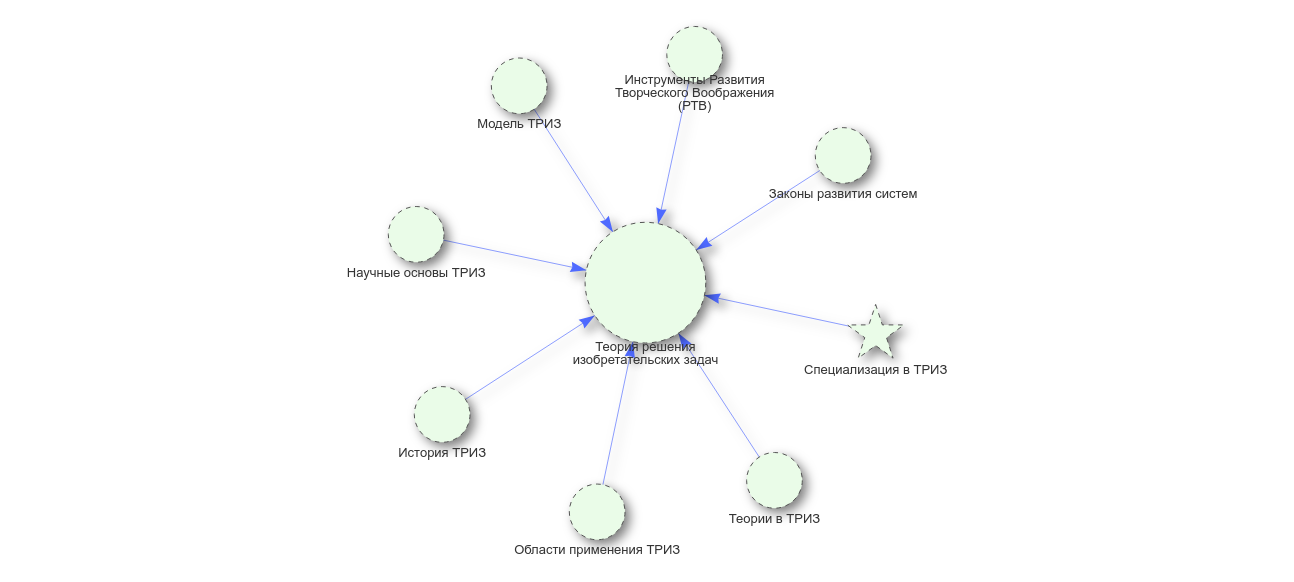
\includegraphics[width=.8\textwidth]{5.png}\\
  Рисунок 5. Онтологическая карта “ТРИЗ” по верхнему уровню.
\end{center}
В целом названия разделов на онтологической карте “ТРИЗ” говорят сами за себя,
мы уточним только отдельные разделы. В раздел “Специализация в ТРИЗ” входят
материалы по методикам и курсам обучения, системам сертификации и информация о
профессиональных объединениях и компаниях в ТРИЗ. Раздел “Модель ТРИЗ”
включает в себя информацию о том, как в ТРИЗ происходит решение
изобретательских задач и развитие систем в целом.

Модель ТРИЗ (рисунок 6) – это схематическое обозначение поэтапного перехода от
задачи к ТРИЗ-модели задачи, затем к ТРИЗ-модели решения и далее к самому
решению. Другой путь в Модели ТРИЗ: от “системы как есть” к ТРИЗ-модели
системы, затем к ТРИЗ-модели новой системы и далее к реальному изменению
системы.  Модель ТРИЗ включает основные компоненты изобретательского мышления:
анализ, синтез, оценка.

\begin{center}
  \addpicture
  Рисунок 6. Визуализация Модели ТРИЗ и соответствующая ей структура модели
  изобретательского мышления.
\end{center}

Онтологическая карта “Модель ТРИЗ” по верхнему уровню отображена на рис. 7.
\begin{center}
  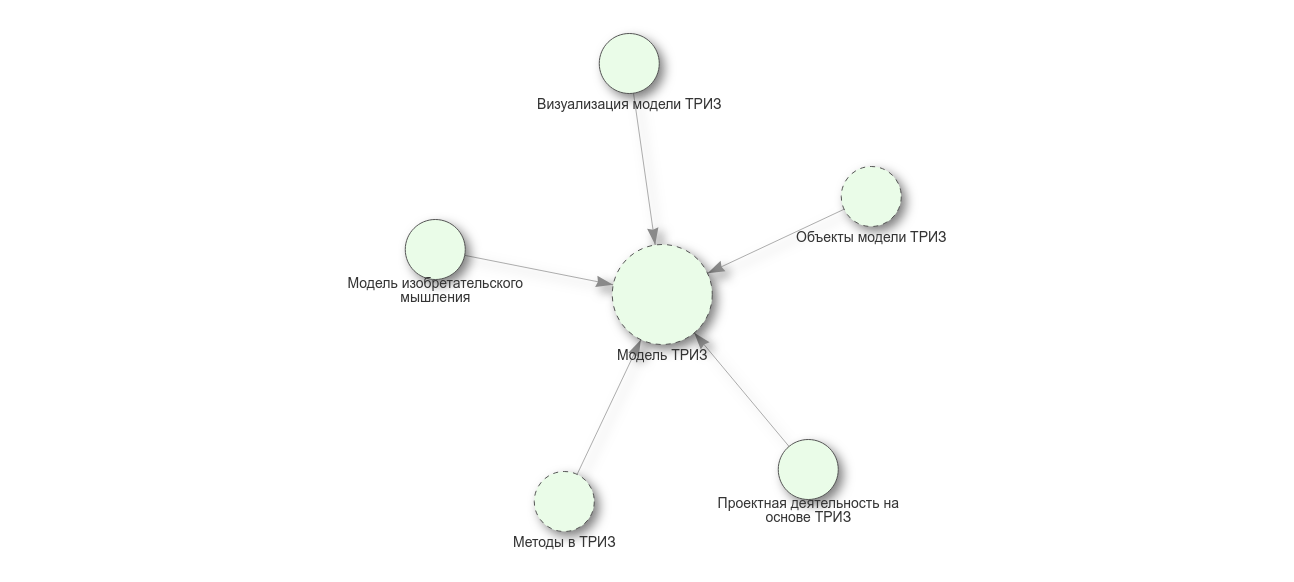
\includegraphics[width=.8\textwidth]{7.png}\\
  Рисунок 7. Онтологическая карта “Модель ТРИЗ”
  \url{https://onto.devtas.ru/new?view=2c3fc934-2486-76ba-4262-ed91a8ca1570}
\end{center}
Онтологическая карта “Модель ТРИЗ” содержит:
\begin{itemize}[noitemsep]
\item примеры визуализации Модели ТРИЗ, например как на рис. 6,
\item объекты модели ТРИЗ (рис. 8)
\item методы преобразования одних объектов модели ТРИЗ в другие.
\end{itemize}
Модель ТРИЗ связана с моделью изобретательского мышления, так как применить на
практике методы ТРИЗ невозможно без соответствующих компонент
изобретательского мышления.

Онтологическая карта “Объекты модели ТРИЗ” отображена на рис. 8.

\begin{center}
  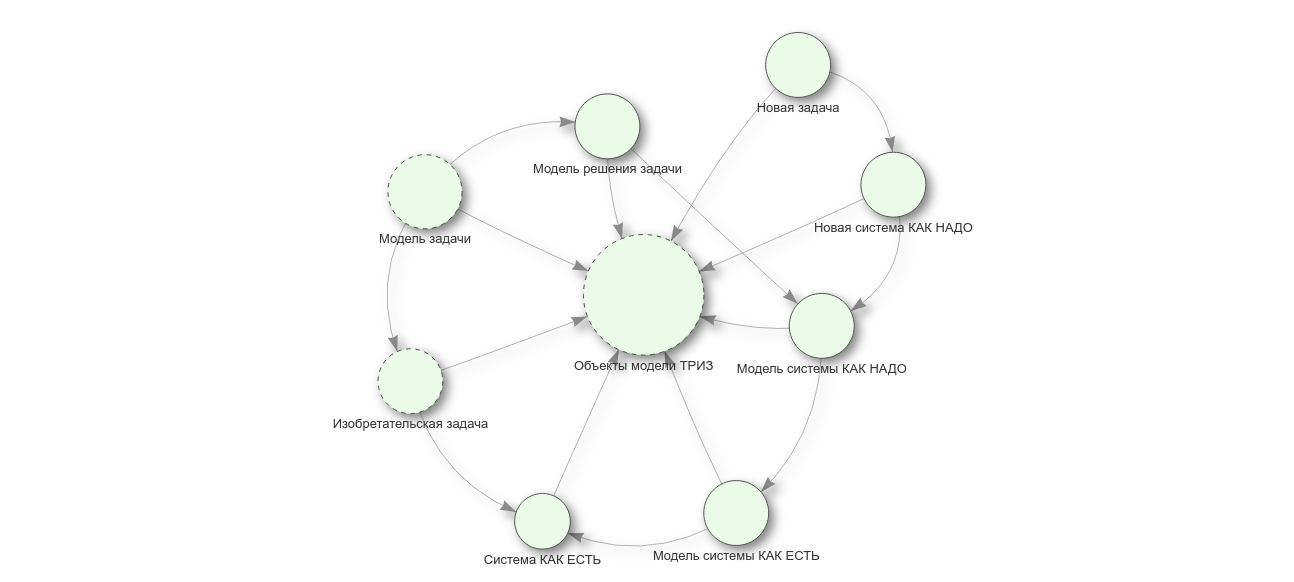
\includegraphics[width=.8\textwidth]{8.png}\\
  Рисунок 8. Онтологическая карта “Объекты модели ТРИЗ”
  \url{https://onto.devtas.ru/new?view=29e5aabb-996c-8fba-1554-b94dacb696ae} 
\end{center}
Из этой карты видно, что “Система КАК ЕСТЬ” может содержать “Изобретательскую
задачу“, может быть преобразована в “Модель системы КАК ЕСТЬ”. “Модель задачи”
получается из “Изобретательской задачи” и может быть преобразована в “Модель
решения задачи”. “Модель системы КАК НАДО” может содержать “Модель решения
задачи” и может быть преобразовано в “Систему КАК НАДО” (синоним “Новая
система”), которая в свою очередь может содержать “Новую задачу”.

Каждый переход от одного объекта Модели ТРИЗ к другому осуществляется
соответствующими методами ТРИЗ, которые описываются в Онтологии “Методы в
ТРИЗ”. Текущее состояние этого
раздела\footnote{\url{https://triz-summit.ru/onto_triz/mod/metod/}} приведено
ниже в тексте этой статьи.

\textbf{Онтология «Методы в ТРИЗ»}
\begin{itemize}
\item Онтология «Методы анализа систем, привнесенные в ТРИЗ»
  \begin{itemize}[noitemsep]
  \item Онтология «MPV анализ»
  \item Онтология «Функционально-стоимостный анализа (ФСА)»
  \item Онтология «Бенчмаркинг»
  \item Онтология «Параметрический анализ»
  \item Онтология «Анализ RCA+»
  \item Онтология «Диаграмма Исикавы»
  \item Онтология «Причинно-следственный анализ»
  \end{itemize}
\item Онтология «Методы анализа систем, разработанные в ТРИЗ»
  \begin{itemize}[noitemsep]
  \item Онтология «Функциональный анализ»
  \item Онтология «Элепольный анализ»
  \item Онтология «Компонентный анализ»
  \item Онтология «Анализ ресурсов»
  \item Онтология «Потоковый анализ»
  \item Онтология «Диверсионный анализ»
  \item Онтология «Структурный анализ»
  \item Онтология «Анализ принципа действия»
  \item Онтология «Анализ по системному оператору»
  \end{itemize}
\item Онтология «Методы преобразования систем»
  \begin{itemize}[noitemsep]
  \item Онтология «Приемы решения противоречий»
  \item Онтология «Метод проб и ошибок»
  \item Онтология «Применение законов и тенденций развития систем»
  \item Онтология «Метод аналогий»
  \item Онтология «Объединение альтернативных систем»
  \end{itemize}
\item Онтология «Методы решения изобретательских задач»
  \begin{itemize}[noitemsep]
  \item Онтология «Принципы решения противоречий»
  \item Онтология «Связь принципов и приемов разрешения противоречий»
  \item Онтология «Таблица применения приемов разрешения противоречий»
  \item Онтология «Элепольные преобразования»
  \item Онтология «Функционально ориентированный поиск (ФОП)»
  \item Онтология «ИКР»
  \end{itemize}
\item Онтология «Методы оценки и развития концепций преобразования систем»
  \begin{itemize}[noitemsep]
  \item Онтология «Сверхэффект»
  \item Онтология «Вторичные задачи»
  \item Онтология «Методы обобщения найденного решения»
  \end{itemize}
\item Онтология «Интегральные методы развития систем»
  \begin{itemize}[noitemsep]
  \item Онтология «АРИЗ»
  \item Онтология «Стандарты на решение изобретательских задач»
  \item Онтология «ТРИЗ-анализ»
  \item Онтология «Связь законов и тенденций с инструментами ТРИЗ»
  \end{itemize}
\end{itemize}
В дальнейшем структура онтологии “Методы в ТРИЗ” будет еще уточняться.

Жизненный цикл ТРИЗ-проектов включает 4 основных этапа:
\begin{itemize}[noitemsep]
\item выявление нежелательных эффектов и предпроектный этап,
\item концептуальный этап,
\item верификацию и
\item внедрение.
\end{itemize}
«Проектная деятельность на основе ТРИЗ» и «Жизненный цикл ТРИЗ-проекта» таким
образом коррелируют с циклом «Модели ТРИЗ» по развитию систем и решению
изобретательских задач. Приведем выдержку из оглавления Онтологии ТРИЗ, с
которой связана онтология “Модель ТРИЗ”:

\textbf{Онтология «Области применения ТРИЗ»}
\begin{itemize}
\item Онтология «Предметные области применения ТРИЗ»
  \begin{itemize}[noitemsep]
  \item Онтология «ТРИЗ в инновационном предпринимательстве»
    \begin{itemize}[noitemsep]
    \item Онтология «Анализ рынка с позиций противоречий и их разрешения»
    \item Онтология «MPV анализ»
    \item Онтология «Анализ потребностей и направлений их развития»
    \end{itemize}
  \item Онтология «ТРИЗ в развитии промышленных предприятий»
  \item Онтология «ТРИЗ в программировании и информационных системах»
  \item Онтология «ТРИЗ в искусстве, литературе и дизайне»
  \item Онтология «ТРИЗ в бизнесе»
  \item Онтология «ТРИЗ в решении научных задач»
  \item Онтология «ТРИЗ в развитии коллективов и социальных систем»
  \end{itemize}
\item Онтология «Проектная деятельность на основе ТРИЗ»
  \begin{itemize}[noitemsep]
  \item Онтология «ТРИЗ в решении изобретательских задач»
  \item Онтология «ТРИЗ в консалтинговой деятельности»
  \item Онтология «ТРИЗ в прогнозировании»
  \item Онтология «Дорожные карты ТРИЗ-проектов»
  \item Онтология «Жизненный цикл ТРИЗ-проекта»
  \end{itemize}
\end{itemize}

Таким образом теоретическая база и методы ТРИЗ непосредственно связаны с
практической проектной деятельностью с применением ТРИЗ при развитии систем и
решении изобретательских задач.

\subsection{Онтология Научные основы ТРИЗ}

В первой же основополагающей публикации по тематике ТРИЗ Г.С. Альтшуллера и
Р.Б. Шапиро «О ПСИХОЛОГИИ ИЗОБРЕТАТЕЛЬСКОГО ТВОРЧЕСТВА» в журнале Вопросы
психологии, No 6 в 1956 году авторы ссылаются на законы диалектики, на научные
исследования в области психологии творчества.

По мере развития ТРИЗ как научной теории расширялись и научные основы ТРИЗ:
системный подход, функциональный подход, эволюционный подход и фундаментальные
научные подходы лежат в основе ТРИЗ.

При этом были разработаны и свои, особенные для ТРИЗ научных подходы в
проведении исследований.

Онтология «Научные основы ТРИЗ» является основой для всей «Онтологии ТРИЗ» в
целом.

В настоящее время в Онтологии “Научные основы ТРИЗ” сформированы следующие
разделы:
\begin{itemize}[noitemsep]
\item Онтология «Диалектика»
\item Онтология «Системный подход»
\item Онтология «Функциональный подход»
\item Онтология «Эволюционный подход»
\item Онтология «Параметрический подход»
\item Онтология «Модельный подход»
\item Онтология «Психология творческого мышления»
\item Онтология «Подходы ТРИЗ»
\item Онтология «Информационные фонды развития систем»
\end{itemize}

\begin{center}
  \addpicture
  Рисунок 9. Ссылка на онтологическую карту “Научные основы
  ТРИЗ”\footnote{\url{https://onto.devtas.ru/new?view=c38a00d7-e97c-9648-bbc2-2af7b21d5d0e}} 
\end{center}

Один из разделов Онтологии “Научные основы ТРИЗ” -- это Онтология «Модельный
подход».  Модель (фр. mod\'ele от лат. modulus «мера, аналог, образец») —
система, исследование которой служит средством для получения информации о
другой системе; представление некоторого реального процесса, устройства или
концепции.  Модель есть абстрактное представление реальности в какой-либо
форме (например, в математической, физической, символической, графической или
дескриптивной), предназначенное для представления определенных аспектов этой
реальности и позволяющее получить ответы на изучаемые вопросы. [Википедия].

Детальнее разделы Онтологии “Научные основы ТРИЗ” опубликованы на на сайте
\url{https://triz-summit.ru/onto_triz/science/}

\subsection{Функция и Функциональный анализ}

В своей основе ТРИЗ опирается на функциональный подход. Понятие «Функция» для
ТРИЗ – одно из центральных понятий. Функция применяется во многих
инструментах: функционально-стоимостной анализ, функциональный анализ,
функционально-идеальное моделирование, функционально-ориентированный поиск и
др.

Онтологически понятие «Функция»[9] связано с Функциональным подходом,
вариантами представления функции, видами и типами (рисунок 7 ?).
\begin{center}
  \addpicture
  Рисунок 10. Онтологическая диаграмма “Функция”
\end{center}
Функция может быть представлена в виде функциональной модели (субъект,
исполнитель действия, -- действие, направленное на изменение параметра, --
объект, параметр которого изменяется), в виде элепольного или, как частного
случая, вепольного представления (рисунок 7?).
\begin{center}
  \addpicture
  Рисунок 11. Онтологическая диаграмма “Тип функции”
\end{center}
По типам функции подразделяются (рисунок 8?) на полезные и вредные, а также в
онтологии выделены в отдельную группу полезные функции с недостатком. К
недостаткам полезных функций относятся избыточность, недостаточность, плохая
управляемость либо отсутствие требуемой функции.

По видам функции подразделяются в зависимости от системного уровня: функции
системы, подсистемы и надсистемы. Также к видам отдельно относятся функции
элемента, как представителя подсистемы, и функции объекта окружающей среды,
как представителя надсистемы.

\begin{center}
  \addpicture
  Рисунок 12. Онтологическая диаграмма “Функция системы”
\end{center}
Функции системы определяют возможности рассматриваемой системы по воздействию
на другие системы в надсистеме (рисунок 9). Главная функция системы – функция,
ради которой создавались система. Главная функция реализует назначение системы
по отношению к надсистеме [2]. Дополнительная функция – функция, не являющаяся
необходимой для обеспечение основного процесса, но которая сопровождает
основную функцию либо помогает достичь её [2]. Латентная функция – функция,
которая не предусматривалась разработчика системы, но которая может
выполняется системой, исходя из потребности пользователя системы.

\begin{center}
  \addpicture
  Рисунок 13. Онтологическая диаграмма “Функция элемента”
\end{center}
Функции элемента определяют возможности рассматриваемого элемента по
воздействию на другие элементы подсистемы либо надсистемы (рисунок 10).
Функции элемента делятся на основные и вспомогательные. Основные функции
направлены на целевой объект воздействия рассматриваемой системы.
Вспомогательная функция направлена на элемент подсистемы либо на элемент
надсистемы, который не является целевым объектом воздействия рассматриваемой
системы. Функции объекта окружающей среды, надсистемы и подсистемы в
описываемой онтологии не классифицированы в настоящий момент.

Как говорилось ранее, понятие «Функция» применяется в различных инструментах
ТРИЗ. На момент написания статьи в системе OSA разработаны онтологические
диаграммы Функционального анализа [10].

Функциональный анализа является частью диаграммы «Методы анализа систем» [11]
(рисунок 11).
\begin{center}
  \addpicture
  Рисунок 14. Онтологическая диаграмма “Методы анализа систем”
\end{center}
\begin{center}
  \addpicture
  Рисунок 15. Онтологическая диаграмма “Функциональный анализ”
\end{center}
Онтологическая диаграмма «Функциональный анализ» (рисунок 12) демонстрирует
связь с целями анализа, моделями функционального анализа, правилами построения
и преобразования моделями, а также показывает два частных случая
функционального анализа: функциональный анализ системы и функциональный анализ
процесса.
\begin{center}
  \addpicture
  Рисунок 16. Онтологическая диаграмма “Цели функционального анализа”
\end{center}
К целям (рисунок 16) функционального анализа относятся:
\begin{itemize}[noitemsep]
\item Выявление и постановка задач;
\item Поиск ресурсов внутри системы или в её окружении;
\item Нахождение новых системных связей;
\item Оценка функциональной модели системы на соответствие требованиям.
\end{itemize}
\begin{center}
  \addpicture
  Рисунок 17. Онтологическая диаграмма “Модели функционального анализа”
\end{center}
Модели функционального анализа (рисунок 17) выбираются в зависимости от вида
анализа. Для функционального анализа системы выбирается функциональная модель
системы, которая строится на основе компонентно-структурной модели с указанием
взаимодействий и их характеристик. Для функциональной модели процесса строится
модель, частным случаем которой является потоковая модель.

Дойдя в онтологической диаграмме Функционального анализа системы до функции,
наблюдатель автоматически попадает на диаграмму функции. Таким образом, нет
необходимости в повторном определении характеристик функций.

\subsection{Поток и Потоковый анализ}

Исходя из определения из глоссария Сушкова [2], \textbf{Потоковый анализ} --
(\emph{перевод с англ.}) аналитический метод и инструмент, который выявляет
недостатки в потоках энергии, веществ и информации в технической системе. В
свою очередь, Олег Герасимов [14] характеризует Потоковый анализ как анализ
технической систем, основанный на выявлении недостатков в потоках Энергии,
Веществ и Информации в пределах Технической Системы, ее серых зон, бутылочных
горлышек, развилок, различных потерь и т.п.

Большинство последующих работ было выполнено Юрием Лебедевым, который вводит
определение потока (ранее отсутствовавшее) как динамического компонента
системы, уточняя, что «Потоки» в технической системе являются специфическими
компонентами. Главная особенность потока как компонента – распределенные (в
пространстве и времени) параметры. Остальные компоненты системы (стационарные)
локализованы в пространстве. Из-за этого отличия потоки крайне неудобно
вписываются в функциональный подход. По этой причине возник специальный
инструмент – потоковый анализ (ПА). В соответствии с этим предлагается
рассматривать потоковый анализ как особый, частный, случай функционального.

Построение онтологической карты позволяет точнее определить потоковый анализ,
а также модель потока в потоковом анализе. Кроме того, показать взаимосвязь
потокового анализа с функциональным анализом и другими понятиями ТРИЗ. С этой
целью были построены две основные онтологические карты: первая --
онтологическая карта «потокового анализа» и вторая -- онтологическая карта
“модели потока”, в развернутом виде, представленные ниже.
\begin{center}
  \addpicture
  Рисунок 18. Онтологическая диаграмма “Потоковый анализ” верхний
  уровень\footnote{\url{https://onto.devtas.ru/new?view=e48bd4bd-3eba-c548-64da-73da1886f744}} 
\end{center}
Видно,
что онтологическая карта меняет понимание целей потокового анализа, переходя
от поиска недостатков к более комплексном цели, где поиск недостатков — это
всего лишь частный случай.

\begin{center}
  \addpicture
  Рисунок 19. Онтологическая диаграмма “Потоковый анализ” часть “Правила
  проведения потокового анализа”
\end{center}
В результате построения онтокарт уточняются следующие определения для модели
потока и потокового анализа.

Потоковый анализ является особым случаем функционального анализа процессов и
служит двум основным целям. Во-первых, описательная цель -- установление
взаимосвязей и поиск ресурсов. Во-вторых, проверка потока на соответствие
требованиям и, как результат, выявление полезных, вредных и паразитных
потоков, а также их изменение. Правила проведения потокового анализа включают
в себя правила оценки модели потока, правила построения модели потока “как
есть”, правила применения закономерности развития потоков в технических
системах, а также, правила построения модели потока на основе соответствия
предъявляемым требованиям. Результатами применения этих правил являются модели
потока “как есть” и “как надо”, а также список задач и противоречий для
последующего решения. Используя приемы изменения потоков, такие, например, как
поиск серой зоны или бутылочного горлышка, можно осуществлять переход от
модели потока “как есть” к модели потока “как надо”.
\begin{center}
  \addpicture
  Рисунок 20. Онтологическая диаграмма “модель
  потока”\footnote{\url{https://onto.devtas.ru/new?view=aacb6c47-827e-b850-7872-978858d06d22}} 
\end{center}
Для описания модели потока выбирается способ описания (чаще всего графический
способ). Далее определяются статические компоненты потока, включающие в себя
систему управления, канал, приемник и источник. Причём система управления может
быть двух типов: насос или вентиль, а источник: источником потенциала или
источником тока.  Важной характеристикой потока в потоковом анализе является
содержание потока, то есть определение того, что течет по каналу, вещество,
энергии и информации. Следующий основной характеристикой является полезность
потока, распределения на полезные вредные или паразитные. Большинство других
характеристик будут выбираться в процессе анализа в зависимости от целей и
содержания потока. Оригинальный тип характеристики функциональность потока,
был изменён на полезность потока, так как функциональность потока связано с
его функции, они с его ценностью для потребителя.

Построение онтологических диаграмм позволяет найти серые зоны и
неформализованные части знаний. В более явном виде показаны связи с другими
знаниями относящимся к ТРИЗ. Следующими шагам могут быть: описание серых зон,
различных правил построения моделей, алгоритмов, а также, матрицы приемов для
перехода от модели (системы) “как есть” к моделе (системе) “как надо”.
Переназвание терминов, для более точного представления сути описываемого
понятия, является также одним из достоинств данного подхода.

\subsection{РТВ -- Курс Развития Творческого Воображения}

Курс Развития Творческого Воображения (дальше РТВ) --
это вспомогательный курс, целью которого является развитие управляемого
воображения, формирование умения преодолевать Психологическую Инерцию в
процессе решения изобретательских
задач\footnote{\url{https://triz-summit.ru/onto_triz/rtv/}}. 
\begin{center}
  \addpicture
  Рисунок 21. Онтологическая диаграмма “Инструменты Развития Творческого
  воображения”
\end{center}
\textbf{Основные отличия курса РТВ:}
\begin{itemize}
\item[1.] Развитие воображения опирается на сознательное использование законов
  развития систем. Так, метод моделирования маленькими человечками основан на
  одной из главных тенденций развития систем -- увеличении степени
  дисперсности рабочих органов. В «Синектике» Гордона используется эмпатия,
  игнорирующая этот закон и потому намного более слабая.
\item[2.] Фантазия рассматривается как вектор (»прыгучесть мысли»): важна не
  только длина прыжка, но и его направление. Курс РТВ нацелен прежде всего на
  получение УПРАВЛЯЕМОЙ ФАНТАЗИИ.
\item[3.] Источниками сильных методов и приемов служат ТРИЗ и «Регистр
  НФ-идей».
\item[4.] Курс РТВ связан с обучением ТРИЗ: акцент сделан на те упражнения,
  которые развивают качества, необходимые для применения ТРИЗ. Вместе с тем
  курс РТВ связан с надсистемой -- развитием сильного мышления: в курс
  включены и упражнения, выходящие за пределы техники.
\item[5.] Обучение -- как и в ТРИЗ -- ведется по принципу: требовать только
  то, чему научили (т.е. не рассчитывать, что слушатель сам по себе -- без
  овладения законами, правилами, методами -- сумеет генерировать сильные
  Ф-идеи).
\end{itemize}
Курс РТВ включает различные методы активизации изобретательского мышления,
предшествовавшие созданию ТРИЗ. Цель их изучения: развитие таких компонентов
изобретательского мышления, как гибкость, вариативность, использование
аналогий, оригинальность; а также изучение этих методов позволяет глубже
понять отличительные особенности ТРИЗ.

\begin{center}
  \addpicture
  Рисунок 22. Онтологическая диаграмма “Методы психологической активизации
  изобретательского мышления”
\end{center}
Мне представляется существенным, что в первой половине 70-х годов на занятиях
были найдены эффективные методы — фантограммы, моделирование маленькими
человечками, поиск икс-фактора на планете, закрытой «условными облаками»,
»золотая рыбка», оператор РВС и др. Особенно важно, по моему мнению, создание
»многоэкранной схемы сильного мышления”\footnote{Альтшуллер Г.С. К истории
  курса РТВ (Справка по курсу РТВ).
  \url{https://www.altshuller.ru/rtv/rtv6.asp}}.
\begin{center}
  \addpicture
  Рисунок 23. Онтологическая диаграмма “Методы Развития Творческого
  Воображения на основе ТРИЗ”.
\end{center}
В курс РТВ включены отдельные инструменты ТРИЗ (Системный Оператор,
Противоречия, ИКР, оператор РВС, ММЧ) с описанием особенностей применения этих
инструментов для развития творческого воображения.
\begin{center}
  \addpicture
  Рисунок 24. Онтологическая диаграмма “Связь с другими разделами ТРИЗ”.
\end{center}
Курс РТВ -- это раздел ТРИЗ, в наибольшей степени связанный с психологией
изобретательского творчества. При формулировке определений для некоторых
терминов использованы материалы по психологии творчества и, в том числе, по
психологии изобретательского творчества.

В частности, термины “Воображение”, “Фантазия”, “Психологическая инерция”
имеют определения, в которых использованы понятия психологии и философии, а
также определения, в которых использованы подходы ТРИЗ.

\begin{center}
  \addpicture
  Рисунок 25. Онтологическая диаграмма “Связь с психологией изобретательского
  творчества”.
\end{center}
Источников методов и приемов Курса РТВ служат ТРИЗ и “Регистр
Научно-Фантастических идей” (далее Регистр НФ-идей). Поэтому некоторые термины
Онтологии Курс РТВ связаны с другими разделами Онтологии ТРИЗ в целом.
Например, термин “Системный оператор”, “Оператор РВС”, “Морфологический
анализ” связаны с аналогичными разделами Онтологии ТРИЗ.

При
составлении программы по Курсу РТВ необходимо учесть две разнонаправленные
линии:
\begin{itemize}
\item необходимо учитывать какие именно компоненты изобретательского мышления
  будут востребованы для изобретательской деятельности конкретного специалиста
  (линия обучения ТРИЗ);
\item в то же время Курс РТВ развивает сильное (изобретательское) мышление в
  целом, и опирается на законы развития мышления (линия развития мышления).
\end{itemize}
На данный момент в Онтологию “Курс Развития Творческого Воображения” вошли
методы “классического” курса. Авторы, работы которых рассматривались при
составлении Онтологии: Г.С. Альтшуллер, П.Р. Амнуэль, М.С. Рубин, С.С. Литвин,
Б.Л.  Злотин, А.В. Зусман, Ю.Г. Тамберг, М.Н. Шустерман, Г.И. Иванов,
И.Н. Мурашковска, Нестеренко А.А., Клемихина Т.В., Крейнина С.В.

\textbf{Дальнейшая работа по Онтологии “Инструменты РТВ”.}
\begin{itemize}
\item Необходимо выстроить связи Онтологии “Курс РТВ” с другими Онтологиями по
  ТРИЗ.
\item Важно разместить переходы к практическому курсу РТВ и диагностическим
  материалам по развитию изобретательского мышления.
\end{itemize}

\subsection{Системный оператор и Анализ по системному оператору}

Системный оператор является частью Онтологии “Системный подход”.
\begin{center}
  \addpicture
  Рисунок 26. Онтологическая диаграмма “Системный подход”.
\end{center}
\begin{center}
  \addpicture
  Рисунок 27. Обобщенная карта “Системный оператор” с сайта Cmaps.
\end{center}
\begin{center}
  \addpicture
  Рисунок 28. Онтологические карты с сайта OSA.
\end{center}
\begin{center}
  \addpicture
  Рисунок 29.  Ссылка на онтологическую карту “Системный
  оператор”\footnote{\url{https://onto.devtas.ru/new?view=938811e9-76cb-6ef3-a2dc-aec74ff3d721}}
\end{center}
Онтология “Анализ по системному оператору” является частью Онтологии “Методы
анализа систем”.
\begin{center}
  \addpicture
  Рисунок 30
\end{center}
Ссылка на онтологическую карту “ТРИЗ” и “Методы анализа систем”
\url{https://onto.devtas.ru/new?view=c38a00d7-e97c-9648-bbc2-2af7b21d5d0e}.

На следующем рисунке показана связь между онтологической карты “Методы анализа
систем” с картой “Анализ по системному оператору”.
\begin{center}
  \addpicture
  Рисунок 31
\end{center}
Ссылка на онтологическую карту “Анализ по системному оператору”:
\url{https://onto.devtas.ru/new?view=a83457ab-77bb-5466-0263-6f4bd5eb3b95}
\begin{center}
  \addpicture
  Рисунок 32.
\end{center}
Работа с онтологией “Системный оператор” позволил лучше выделить особенности
этого инструмента ТРИЗ, его связь с системным подходом, законами развития
систем, курсом “Развития творческого воображения”. Выделены области роста в
методиках построения и применения системного оператора, начались разработки по
анализу вариативности переходов по экранам системного оператора, методике
итерационных изменений экранов, пространственный системный оператор и другие
направления развития системного оператора и анализу по системному оператору.

Следующие шаги: 
\begin{itemize}
\item Завершить строительство структуры онтологических карт «Системный
  оператор» и «Анализ по системному оператору».
\item Развивать методики применения системного оператора для решения
  изобретательских задач и для прогнозирования развития систем.
\item Выделить общее в построении онтологических карт различных методов
  анализа из Онтологии «Методы анализа систем».
\end{itemize}

\section{Проект ТРИЗ онтология}
\subsection{Цели и задачи проекта}

Проект по созданию онтологии ТРИЗ был инициирован в 2019 году группой
специалистов по ТРИЗ: Андрей Курьян, Валерий Сушков, Дмитрий Кучерявый, Михаил
Рубин, Николай Щедрин в рамках ТРИЗ Саммит 2019 на основании доклада [8].

Целями проекта являются:
\begin{itemize}
\item[] В отношении существующего Глоссария ТРИЗ:
  \begin{itemize}[noitemsep]
  \item проверить правильность каждого термина в существующем Глоссарии ТРИЗ;
  \item уточнить термины и определения в существующем Глоссарии ТРИЗ;
  \item обнаружить и устранить пробелы в существующем Глоссарии ТРИЗ.
  \end{itemize}
\item[]   В отношении ТРИЗ в целом:
  \begin{itemize}[noitemsep]
  \item улучшить качество обучения и понимания ТРИЗ;
  \item помочь избежать неправильного использования и неправильного толкования
    терминов ТРИЗ;
  \item избегать введения новых терминов без необходимости;
  \item выявить несоответствия в использовании терминов ТРИЗ;
  \item способствовать развитию теории, которая может обеспечить
    количественную предсказательную силу;
  \item помочь в интеграции ТРИЗ с другими доменами или внутри них.
  \end{itemize}
\item[] В рамках проекта предусматривается:
  \begin{itemize}[noitemsep]
  \item[1)] Выделение ключевых понятий ТРИЗ, которые связаны с другими
    понятиями ТРИЗ различными отношениями.
  \item[2)] Разработка онтологических диаграмм, отображающих связи между
    понятиями ТРИЗ.
  \item[3)] Обсуждение онтологических диаграмм в кругу ТРИЗ специалистов.
  \item[4)] Разработка новых определений понятий ТРИЗ на основе онтологии
    ТРИЗ. 
  \end{itemize}
\end{itemize}
Проект является открытым, т.е., каждый специалист ТРИЗ может принять участие в
проекте, в том числе, разрабатывать онтологические диаграммы, обсуждать уже
созданные онтологические диаграммы или определения понятий ТРИЗ.

\subsection{Сайт OSA}
Выбор среды, в которой будут создаваться онтологические диаграммы, -- один из
важнейших шагов проекта по созданию онтологии. Среда разработки должна иметь
удобный и понятный интерфейс, иметь достаточный функционал для построения
связей и их описания. Она должна позволять применять построенные диаграммы в
различных системах, для чего программный комплекс должен содержать API.

Для разработки онтологии области знаний Теории решения изобретательских задач
была выбрана платформа OSA – Ontology Space Agent (редактор коллективной
разработки и согласования, тестирование онтологий, машина вывода) [12],
разработанная специалистами российской компании «Time \& Space» [13].

Преимуществами платформы являются:
\begin{itemize}[noitemsep]
\item возможность интегрирования с другими платформами,
\item возможность создания глоссария, документации на основе онтологических
  диаграмм,
\item наличие чата с настройкой личных или групповых сообщений,
\item возможность прямой связи с разработчиками
\item и др.
\end{itemize}

\begin{center}
  \addpicture
  Рисунок 33. Стартовая страница
\end{center}
\begin{center}
  \addpicture
  Рисунок 34. Главная страница
\end{center}
Платформа OSA отличается удобным интерфейсом. На стартовой странице
онтологическая платформа предлагает пользователю пройти авторизацию (рис. 26).
После ввода учетных данных пользователь попадает на главную страницу
(рис. 27).  Главная страница отображает список событий проекта, позволяет
перейти в настройки рабочих сессий и установить задачи проекта, отправлять
сообщения другим пользователям, изменить персональные данные и перейти к
созданию и редактированию онтокарт.
\begin{center}
  \addpicture
  Рисунок 35. Рабочее поле
\end{center}
\begin{center}
  \addpicture
  Рисунок 36. Поле построения суждения
\end{center}
\begin{center}
  \addpicture
  Рисунок 37. Настройки суждения
\end{center}
При переходе на страницу редактора онтокарт перед пользователем появляется
рабочее поле, на котором строятся онтологические связи (рисунок 28). Перед
редактированием есть возможность открыть готовую онтокарту либо начать
создание новой. В поле построения суждения указываются два объекта и связь
между ними (рисунок 29), при этом параметры связи могут быть настроены
(рисунок 30).  Платформа позволяет создавать и сохранять связи в различных
областях. Например, создавая онтокарту ТРИЗ-инструмента, пользователь помещает
данную карту в область ТРИЗ. При необходимости связи могут быть отнесены сразу
к нескольким областям. Такое понятие, как требование, может быть отнесено к
области ТРИЗ и области Управления требованиями. Указание областей позволяет
осуществлять переход от одной диаграммы к другой в рамках одной предметной
области, без перескоков на другие.
\begin{center}
  \addpicture
  Рисунок 38. Список терминов
\end{center}
После создания диаграммы OSA позволяет наполнить глоссарий терминов, которые
использовались в диаграмме. Список терминов формируется автоматически
(рис. 31).  Если в какой-либо области термин определен, то определение также
автоматически подгружается в глоссарий с указанием предметной области.
\begin{center}
  \addpicture
  Рисунок 39. Переход между диаграммами
\end{center}
Если в системе присутствуют несколько онтокарт, содержащих одинаковые объекты,
платформа OSA отображает возможность перехода с карты на карту. Совпадающие
объекты выделяются пунктирной линией (рисунок 32). Подобная функция системы
позволяет выходить на другие области знаний, которые используют те же понятия,
что и ТРИЗ, и выявлять общность и различия.

Онтологическая платформа OSA является удобным и эффективным инструментом
построения онтологий области знаний Теории решения изобретательских задач,
позволяющая находить пересечения с другими областями и дисциплинами, выявлять
новые связи, детальнее разобраться, а иногда и переосмыслить, привычные
термины и инструменты. В дальнейшем ожидается, что платформа позволит создать
полноценную базу знаний по ТРИЗ и откроет возможности автоматизированной
разработки индивидуальных курсов подготовки специалистов по ТРИЗ.

\subsection{Сайт triz-summit.ru}

Разработка Онтологии ТРИЗ идет с применением трех инструментов.
Предварительная, общая картина конкретного онтологического раздела готовится
на специализированном сайте \url{https://onto.devtas.ru/ts2o1}.
\begin{center}
  \addpicture
  Рисунок 40.
\end{center}
Далее, эти связи переносятся на онтологические карты в системе OSA, о которой
уже было сказано выше и с которой можно познакомиться по ссылке
\url{https://onto.devtas.ru/new?view=c38a00d7-e97c-9648-bbc2-2af7b21d5d0e}

Для повышения доступности разработок по проекту “Онтология ТРИЗ” и организации
обсуждения вся информация по проекту публикуется на сайте сайте Саммита
разработчиков ТРИЗ \url{https://triz-summit.ru/onto_triz/}.

В этом разделе мы кратко опишим содержание и роль этого сайте в проекте
“Онтология ТРИЗ”.
\begin{center}
  \addpicture
  Рисунок 41.
\end{center}

Перечень разделов страницы проекта “Онтология ТРИЗ” приведен на рисунке с
копией экрана с сайта:
\begin{itemize}[noitemsep]
\item Онтология «Научные основы ТРИЗ»
\item Онтология «Области применения ТРИЗ»
\item Онтология «Законы развития систем» 
\item Онтология «Методы анализа систем»
\item Онтология «Методы преобразования систем»
\item Онтология «Методы решения изобретательских задач»
\item Онтология «Методы оценки и развития концепций преобразования систем»
\item Онтология «Интегральные методы развития систем»
\item Онтология «Теории в ТРИЗ»
\item Онтология «Курс Развития Творческого Воображения (РТВ)»
\item Онтология «Специализация в ТРИЗ»
\item Онтология «История ТРИЗ»
\item О проекте Онтология ТРИЗ
\end{itemize}
Все основные страницы с описанием
онтологий тех или иных понятий строятся примерно по единой форме. На странице
описывается: 
\begin{itemize}[noitemsep]
\item иерархия данного понятия в Онтологии ТРИЗ,
\item определение по глоссарию терминов Сушкова В. (перевод на русский язык)
\item Изменения, дополнения или уточнения. Предложение нового определения.
\end{itemize}
Синонимы.  
\begin{itemize}
\item Дается перечень и ссылки на зависимые термины и понятия 
\item Приводятся онтологические карты со ссылкой на сайт OSA.
\end{itemize}
Приведем несколько примеров.

Описание на сайте Онтологии «Административное противоречие (проблемная
ситуация)»
\url{https://triz-summit.ru/onto_triz/science/triz_ap/invent/contradict/adm/}:
\begin{center}
  \addpicture
  Рисунок 42.
\end{center}
Описание на сайте Онтологии “Системный оператор”
\url{https://triz-summit.ru/onto_triz/science/sys/sys_op/}:
\begin{center}
  \addpicture
  Рисунок 43.
\end{center}
Если вводятся новые понятия, то готовится и публикуется для обсуждения
обоснование введения нового термина или понятия. Например, на сайте
опубликовано обоснование введения понятия “Вариативность системных переходов”
\url{https://triz-summit.ru/onto_triz/science/sys/sys_op/svayz/var/}. На этой
странице дается:
\begin{itemize}
\item иерархический путь к этому понятию: Главная $\to$ Онтология ТРИЗ $\to$
  Онтология «Научные основы ТРИЗ» $\to$ Онтология «Системный подход» $\to$
  Онтология «Системный оператор» $\to$ Онтология «Связи между экранами»
\item дается краткое описание и примеры использования
\item дается обоснование необходимости введения этого понятия (инструмента,
  элемента анализа и т.д.)
\item публикуется иллюстративный материал:
\end{itemize}
\begin{center}
  \begin{quote}
    Вариабельность переходов по системному оператору. Филогенез, прошлое. Путь
    через надсистему и через прошлое приводит к разным результатам. 
  \end{quote}
  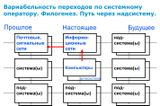
\includegraphics[width=.4\textwidth]{44-1.jpeg}\hfill 
  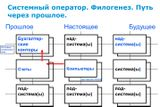
\includegraphics[width=.4\textwidth]{44-2.jpeg} 
  \begin{quote}
    Вариабельность системного оператора. Прогнозирование. Путь через надсистему и
    по горизонтали. 
  \end{quote}
  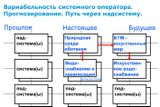
\includegraphics[width=.4\textwidth]{44-3.jpeg}\hfill 
  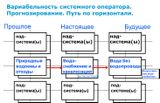
\includegraphics[width=.4\textwidth]{44-4.jpeg} 
 
  Рисунок 44. Иллюстрации к статье “Вариативность системных переходов”
\end{center}
Приведем фрагмент структуры проекта “Онтология ТРИЗ” на сайте:
\begin{center}
  \addpicture
  Рисунок 45. Фрагмент Онтологии ТРИЗ на сайте
  \url{https://triz-summit.ru/Onto_TRIZ/}
\end{center}
Следующие шаги и планы на будущее: 
\begin{itemize}
\item Завершить строительство структуры раздела «Онтология ТРИЗ» на сайте.
\item Обновить определения терминов и ссылки на онтологические карты.
\item Организовать обратную связь для обсуждения разделов и терминов
  «Онтологии ТРИЗ» и развития проекта в целом.
\item Ввести классификационный индекс материалов по ТРИЗ в соответствии с
  онтологией ТРИЗ.
\item Скорректировать систему «Икар и Дедал» в соответствии с Онтологией
  ТРИЗ. 
\item Разработать путеводитель по сайту Сайт TRIZ Summit в соответствии с
  индексом материалов по ТРИЗ.
\end{itemize}

\subsection{Как организован проект}

Для реализации проекта по созданию Онтологии ТРИЗ создана открытая платформа.
Она включает:
\begin{itemize}
\item[1.] отдельную платформу OSA для разработки и хранения онтологических
  диаграмм;
\item[2.] раздел “Онтология ТРИЗ” на сайте triz-summit.ru (далее сайт
  Онтологии ТРИЗ), где находятся описания Онтологии ТРИЗ.
\end{itemize}
На следующем рисунке представлена структурная схема платформы для Онтологии
ТРИЗ.
\begin{center}
  \addpicture
  Рисунок 46. Платформа для проекта “Онтология ТРИЗ”
\end{center}
В следующей таблице представлено описание
ответственности заинтересованных сторон проекта Онтология ТРИЗ.
\begin{center}
  \begin{tabular}{|l|p{12cm}|}\hline
    Модератор & участник команды Онтология ТРИЗ. Он отвечает за создание задач
    по разработке частей онтологии для Экспертов, а также за контроль
    выполнения этих задач.\\\hline
    Эксперт & участник команды Онтология ТРИЗ. Он отвечает за создание
    онтологических диаграмм и их описаний.\\\hline
    Визитер & это любой человек, который интересуется областью знаний ТРИЗ в
    целом и, в частности, Онтологией ТРИЗ. Визитер может изучать
    онтологические диаграммы и их описания на сайте triz-summit.ru, принимать
    участие в дискуссиях и высказывать свои мнения и оценки. \\\hline
  \end{tabular}
\end{center}
На сайте проекта “Онтология ТРИЗ” дается также описание проекта, есть раздел
“Инструкция для участников проекта” и раздел “Предложения онтологии ТРИЗ”
\url{https://triz-summit.ru/onto_triz/proj/predl/}

\begin{center}
  \addpicture
  Рисунок 47.
\end{center}
\begin{center}
  \addpicture
  Рисунок 48.
\end{center}
\begin{center}
  \addpicture
  Рисунок 49.
\end{center}

\section{Заключение}

Онтология ТРИЗ -- это сегодня необходимый шаг для развития ТРИЗ. Она является
фундаментом, на котором должна строиться новая версия области знаний ТРИЗ.

Создание Онтологии ТРИЗ невозможно без участия широких кругов специалистов
ТРИЗ. Авторы доклада призывают всех заинтересованных лиц подключаться к
проекту по созданию Онтологии ТРИЗ.

\section{Ссылки}
\begin{itemize}[leftmargin=18pt]
\item[1.] Альтшуллер Г.С. Справка ТРИЗ-88.\\
  \url{https://www.altshuller.ru/engineering/engineering16.asp}
\item[2.] Souchkov V. Glossary of TRIZ and TRIZ-related terms.  ver. 1.2.
  MATRIZ-2018.\\
  \url{https://matriz.org/wp-content/uploads/2016/11/TRIZ-Glossary.pdf}
\item[3.] Литвин С., Петров В., Рубин М. Основы знаний по ТРИЗ. Версия
  1.0. 2007.\\ \url{https://triz-summit.ru/triz/metod/basics/1/203703/}
\item[4.] MATRIZ Regulations for Multi-Level Certification of TRIZ Users and
  Specialists.  MATRIZ, 2016.
\item[5.] Хоменко Н.Н. ОТСМ-ТРИЗ
\item[6.] Рубин М.С. Эволюционное системоведение.\\
  \url{https://triz-summit.ru/triz/metod/evos/}
\item[7.] Международная система оценки знаний и навыков ТРИЗ “Икар и
  Дедал”.\\ \url{https://triz-summit.ru/certif/}
\item[8.] Kuryan A., Souchkov V., Kucharavy D. Towards ontology of TRIZ.
  Proceedings of TRIZ Developers Summit 2019 Conference, Minsk, 2019.\\
  \url{https://triz-summit.ru/confer/tds-2019/articles/it/}
\item[9.]
  \url{https://triz-summit.ru/onto_triz/analysis/fa/model_fa/func_syst_model/func/} 
\item[10.] \url{https://triz-summit.ru/onto_triz/analysis/fa/}
\item[11.] \url{https://triz-summit.ru/onto_triz/analysis/}
\item[12.] \url{https://devtas.ru/docs/}
\item[13.] \url{http://tas-project.ru/}
\item[14.] \texttt{https://triz.ao-npk.ru/wp-content/uploads/2020/05/Потоковый-Анализ-для-Вебинара.pdf}
\end{itemize}
\end{document}
